% Provenance (never printed): see sources/outline_sources.md and sources/book1/BRIEFS.md (g3/02).
\chapter{Inside the Computer}\label{ch:g3:inside-the-computer}

The school has a new \omterm{def:g1:what-is-a-computer:computer}{computer}, so the teacher brings the old one into the
classroom, lays it on her desk and unscrews its side. Inside there are wires of
many colours, a fan, a big green board covered with tiny parts, and a few small
black squares. ``Somewhere in here,'' she says, ``are the parts that follow the
\omterm{def:g1:instructions-in-order:instruction}{instructions}, the parts that remember, and the parts that keep your work when
the power is off. Let us find them.''

\begin{omfigure}
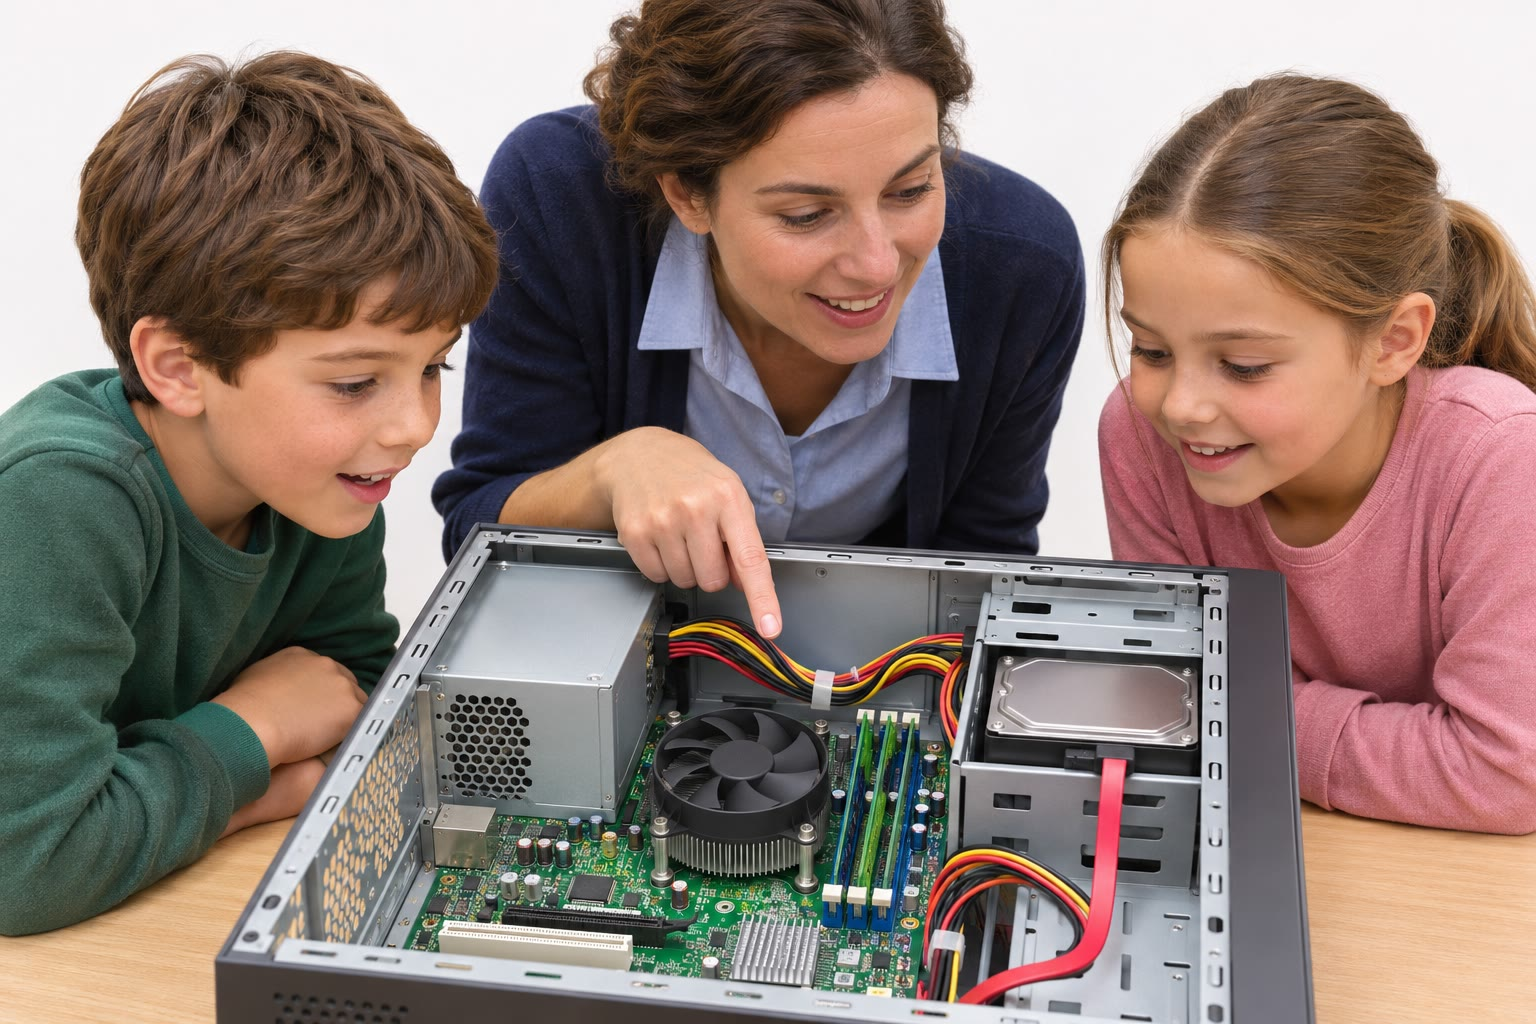
\includegraphics[width=0.6\linewidth]{images/book1/ai/g3-inside-the-computer-open-case.jpg}

{\small An old desktop \omterm{def:g1:what-is-a-computer:computer}{computer}, opened on the teacher's desk.}
\end{omfigure}

\begin{recall}
A \omterm{def:g1:what-is-a-computer:computer}{computer} is a machine that follows \omterm{def:g1:instructions-in-order:instruction}{instructions} to work on information.
\omterm{def:g1:what-is-a-computer:device}{Input devices} bring information in; \omterm{def:g1:what-is-a-computer:device}{output devices} take it out
(\cref{ch:g1:what-is-a-computer}).
\end{recall}

\section{The processor}

\begin{definition}[Processor]\label{def:g3:inside-the-computer:processor}
The \emph{processor}\index{processor} is the part of a \omterm{def:g1:what-is-a-computer:computer}{computer} that carries
out the \omterm{def:g1:instructions-in-order:instruction}{instructions}, one after another, very fast.
\end{definition}

The \omterm{def:g3:inside-the-computer:processor}{processor} is a small, flat square, a few centimetres wide, made of
silicon and covered by a metal lid. It carries out hundreds of millions of
\omterm{def:g1:instructions-in-order:instruction}{instructions} every second. All this work makes it hot, so a fan or a block of
metal with fins sits on top of it to carry the heat away.

\section{The memory}

To work on a drawing, the \omterm{def:g3:inside-the-computer:processor}{processor} needs it close at hand. The drawing you
are working on, and the \omterm{def:g1:instructions-in-order:instruction}{instructions} of the tool you are using, are kept in
the \omterm{def:g3:inside-the-computer:memory}{memory} while you work.

\begin{definition}[Memory]\label{def:g3:inside-the-computer:memory}
The \emph{memory}\index{memory (of a computer)} of a \omterm{def:g1:what-is-a-computer:computer}{computer} holds the
information the \omterm{def:g1:what-is-a-computer:computer}{computer} is working on right now: the open work and the
\omterm{def:g1:instructions-in-order:instruction}{instructions} being carried out. It forgets everything when the power goes off.
\end{definition}

The \omterm{def:g3:inside-the-computer:memory}{memory} is very fast: the \omterm{def:g3:inside-the-computer:processor}{processor} reads from it and writes into it all the
time. But it needs electricity to remember. This is why Sami's castle (\cref{ch:g2:using-a-computer}) was
lost: it was only in the \omterm{def:g3:inside-the-computer:memory}{memory} when the \omterm{def:g1:what-is-a-computer:computer}{computer} was switched off.

\section{The storage}

\begin{definition}[Storage]\label{def:g3:inside-the-computer:storage}
The \emph{storage}\index{storage} of a \omterm{def:g1:what-is-a-computer:computer}{computer} keeps information when the
power is off: the saved work and the tools installed on the \omterm{def:g1:what-is-a-computer:computer}{computer}.
\end{definition}

When you save a drawing, the \omterm{def:g1:what-is-a-computer:computer}{computer} copies it from the \omterm{def:g3:inside-the-computer:memory}{memory} into the
\omterm{def:g3:inside-the-computer:storage}{storage}. When you open it the next day, the \omterm{def:g1:what-is-a-computer:computer}{computer} copies it back from the
\omterm{def:g3:inside-the-computer:storage}{storage} into the \omterm{def:g3:inside-the-computer:memory}{memory}, so that you can go on working. The next year will
show what is inside the \omterm{def:g3:inside-the-computer:storage}{storage} of a \omterm{def:g1:what-is-a-computer:computer}{computer}.

\begin{example}[Memory or storage?]\label{ex:g3:inside-the-computer:which}
Mia is writing a story that she has not saved yet: the story is only in the
\omterm{def:g3:inside-the-computer:memory}{memory}. She saves it: now a copy is also in the \omterm{def:g3:inside-the-computer:storage}{storage}. The power goes off
by accident: the copy in the \omterm{def:g3:inside-the-computer:memory}{memory} is lost, but the saved copy in the \omterm{def:g3:inside-the-computer:storage}{storage}
is still there. Only the words she typed after saving are lost.
\end{example}

\begin{omfigure}
\begin{tikzpicture}[x=1cm, y=1cm, font=\small,
    part/.style={draw=black!70, rounded corners=3pt, minimum width=2.8cm, minimum height=1.1cm, align=center},
    arr/.style={{Stealth[length=2.2mm]}-{Stealth[length=2.2mm]}, thick, black!60},
    one/.style={-{Stealth[length=2.2mm]}, thick, black!60}]
  \node[part, fill=ocRed!20] (cpu) at (4.5,2.2) {processor\\{\footnotesize carries out instructions}};
  \node[part, fill=ocBlue!20] (mem) at (0,2.2) {memory\\{\footnotesize work in progress}};
  \node[part, fill=ocMint!25] (sto) at (9,2.2) {storage\\{\footnotesize saved work}};
  \node[part, fill=ocYellow!35] (in) at (2.2,0) {input devices\\{\footnotesize keyboard, mouse}};
  \node[part, fill=ocYellow!35] (out) at (6.8,0) {output devices\\{\footnotesize screen, speakers}};
  \draw[arr] (mem) -- (cpu);
  \draw[arr] (cpu) -- (sto);
  \draw[one] (in) -- (cpu);
  \draw[one] (cpu) -- (out);
  \draw[black!40, dashed, rounded corners=6pt] (-1.7,1.35) rectangle (10.7,3.15);
  \node[anchor=south west, font=\footnotesize, text=black!60] at (-1.7,3.15) {on the motherboard, inside the case};
\end{tikzpicture}

{\small The main parts of a \omterm{def:g1:what-is-a-computer:computer}{computer} and how information moves between them.
\omterm{def:g1:what-is-a-computer:input}{Input} comes in through the ports, the \omterm{def:g3:inside-the-computer:processor}{processor} works with the \omterm{def:g3:inside-the-computer:memory}{memory}, saved
work goes to the \omterm{def:g3:inside-the-computer:storage}{storage}, and \omterm{def:g1:what-is-a-computer:input}{output} goes out through the ports.}
\label{fig:g3:inside-the-computer:blocks}
\end{omfigure}

\section{The motherboard, the power and the heat}

\begin{definition}[Motherboard]\label{def:g3:inside-the-computer:motherboard}
The \emph{motherboard}\index{motherboard} is the large board inside a
\omterm{def:g1:what-is-a-computer:computer}{computer} to which all the parts are attached. Tiny copper paths on the board
carry information and electricity from one part to another.
\end{definition}

The \omterm{def:g3:inside-the-computer:processor}{processor} sits in a socket on the \omterm{def:g3:inside-the-computer:motherboard}{motherboard}. The \omterm{def:g3:inside-the-computer:memory}{memory} is made of thin
sticks clipped into long slots. The \omterm{def:g3:inside-the-computer:storage}{storage} is a box or a small card connected
to the \omterm{def:g3:inside-the-computer:motherboard}{motherboard}. A desktop \omterm{def:g1:what-is-a-computer:computer}{computer} gets its electricity from a power supply
plugged into the wall; a laptop, a tablet or a phone from a battery, which is
charged when it is plugged in.

\begin{omfigure}
\begin{tikzpicture}[x=1cm, y=1cm, font=\footnotesize, lab/.style={font=\footnotesize, anchor=west}]
  % case
  \draw[black!70, fill=black!6, rounded corners=3pt] (0,0) rectangle (7,8);
  % motherboard
  \draw[black!60, fill=ocMint!35] (0.6,2.4) rectangle (5.4,7.4);
  \foreach \x/\y in {0.9/2.7, 1.5/3.3, 2.4/2.8, 4.9/3.1, 5.0/6.8, 0.9/5.6}
    \draw[ocMint!80!black] (\x,\y) -- ++(0.6,0) -- ++(0,0.3);
  % processor + fan
  \draw[black!70, fill=black!25] (1.3,5.0) rectangle (2.9,6.6);
  \draw[black!70, fill=white] (2.1,5.8) circle (0.68);
  \foreach \a in {0,72,...,288} \draw[black!60, fill=black!15] (2.1,5.8) -- ++(\a:0.6) arc[start angle=\a, end angle=\a+40, radius=0.6] -- cycle;
  % memory sticks
  \foreach \x in {3.5,3.85,4.2} \draw[black!70, fill=ocBlue!45] (\x,4.6) rectangle ++(0.22,2.4);
  % storage
  \draw[black!70, fill=black!30, rounded corners=2pt] (5.7,4.3) rectangle (6.8,6.1);
  \draw[black!50] (5.75,4.9) -- (5.4,4.9);
  % power supply
  \draw[black!70, fill=black!35] (0.4,0.3) rectangle (3.2,1.9);
  \draw[black!60, fill=white] (1.8,1.1) circle (0.55);
  \foreach \a in {0,60,...,300} \draw[black!40] (1.8,1.1) -- ++(\a:0.5);
  % cables
  \draw[ocRed!70, line width=1pt] (3.2,1.3) .. controls (4.2,1.4) and (4.6,2.0) .. (4.7,2.5);
  \draw[ocYellow!80!black, line width=1pt] (3.2,1.0) .. controls (5.2,1.1) and (6.2,2.5) .. (6.2,4.3);
  % ports at the back (left edge)
  \foreach \y in {5.4,5.8,6.2,6.6} \draw[black!70, fill=white] (0.05,\y) rectangle (0.45,\y+0.22);
  % labels
  \draw[black!60] (2.1,6.48) -- (7.4,7.6) node[lab] {processor, under its fan};
  \draw[black!60] (4.2,6.5) -- (7.4,6.9) node[lab] {memory sticks};
  \draw[black!60] (6.8,5.2) -- (7.4,5.6) node[lab] {storage};
  \draw[black!60] (5.2,3.4) -- (7.4,3.4) node[lab] {motherboard};
  \draw[black!60] (3.0,1.6) -- (7.4,1.6) node[lab] {power supply, with its fan};
  \draw[black!60] (0.25,6.0) -- (-0.6,6.0) node[anchor=east] {ports};
\end{tikzpicture}

{\small The inside of a desktop \omterm{def:g1:what-is-a-computer:computer}{computer}, drawn from the side. All the parts are
attached to the \omterm{def:g3:inside-the-computer:motherboard}{motherboard}; the power supply brings electricity through the
cables.}
\label{fig:g3:inside-the-computer:case}
\end{omfigure}

\begin{omfigure}
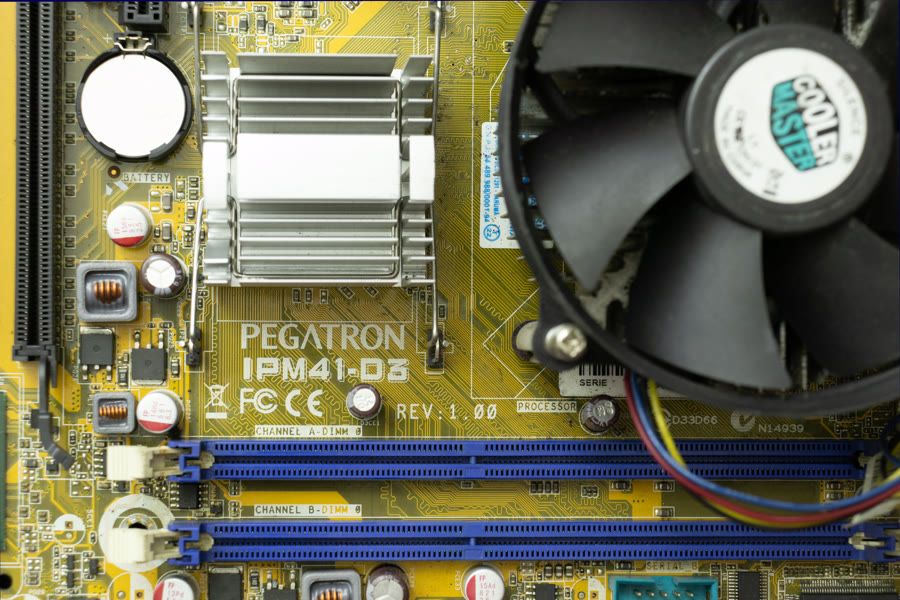
\includegraphics[width=0.62\linewidth]{images/book1/g3-motherboard.jpg}

{\small Part of a real \omterm{def:g3:inside-the-computer:motherboard}{motherboard}. On the right, the fan that cools the
\omterm{def:g3:inside-the-computer:processor}{processor}; below, two long blue slots for \omterm{def:g3:inside-the-computer:memory}{memory} sticks; in the middle, a metal
block with fins that carries heat away from another chip. Photograph: Davidson
F, CC0.}
\end{omfigure}

Every part of a working \omterm{def:g1:what-is-a-computer:computer}{computer} turns a little electricity into heat. Fans
blow cool air in through holes in the case, the vents, and push warm air out.
If the vents are covered, by a blanket or a cushion under a laptop, the heat
cannot get out: the \omterm{def:g1:what-is-a-computer:computer}{computer} becomes very hot and slows down to protect itself.

\begin{safety}
Never cover the vents of a \omterm{def:g1:what-is-a-computer:computer}{computer}: keep a laptop on a table, not on a bed or
a cushion. Never open the case of a \omterm{def:g1:what-is-a-computer:computer}{computer} that is plugged in, and never
open the power supply or a battery.
\end{safety}

\section{Ports and devices}

\begin{definition}[Device]\label{def:g3:inside-the-computer:device}
A \emph{device}\index{peripheral device} is a part that is connected to a
\omterm{def:g1:what-is-a-computer:computer}{computer} from the outside: a mouse, a keyboard, a screen, a printer,
headphones, a camera, a \omterm{def:g3:inside-the-computer:memory}{memory} stick. It is plugged into a socket of the
\omterm{def:g1:what-is-a-computer:computer}{computer}, called a port, or connected by radio, without a cable.
\end{definition}

Each port has a shape, so that only the right plug fits into it. Some ports
carry information in, some carry it out, and many carry both. A wireless mouse
or wireless headphones use radio instead of a cable, but they are \omterm{def:g3:inside-the-computer:device}{devices} all
the same. Some ports also carry electricity: the cable that charges a phone is
plugged into a port.

\begin{omfigure}
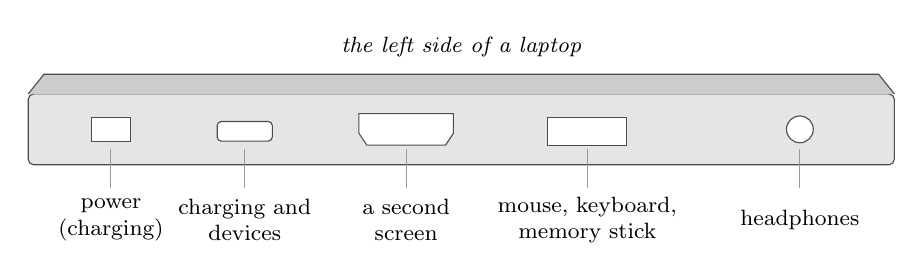
\begin{tikzpicture}[x=1cm, y=1cm, font=\footnotesize, lab/.style={font=\footnotesize, align=center}]
  % laptop seen from the side: its left edge
  \draw[black!70, fill=black!10, rounded corners=2pt] (0,0) rectangle (11,0.9);
  \draw[black!70, fill=black!20] (0,0.9) -- (0.2,1.15) -- (10.8,1.15) -- (11,0.9);
  % ports
  \draw[black!70, fill=white] (0.8,0.3) rectangle (1.3,0.6);                      % power
  \draw[black!70, fill=white, rounded corners=1.5pt] (2.4,0.3) rectangle (3.1,0.55); % small flat port
  \draw[black!70, fill=white] (4.3,0.25) -- (5.3,0.25) -- (5.4,0.4) -- (5.4,0.65) -- (4.2,0.65) -- (4.2,0.4) -- cycle; % screen port
  \draw[black!70, fill=white] (6.6,0.25) rectangle (7.6,0.6);                     % rectangular port
  \draw[black!70, fill=white] (9.8,0.45) circle (0.17);                          % headphones
  % labels
  \node[lab] at (1.05,-0.7) {power\\(charging)};
  \node[lab] at (2.75,-0.7) {charging and\\devices};
  \node[lab] at (4.8,-0.7) {a second\\screen};
  \node[lab] at (7.1,-0.7) {mouse, keyboard,\\memory stick};
  \node[lab] at (9.8,-0.7) {headphones};
  \foreach \x in {1.05,2.75,4.8,7.1,9.8} \draw[black!40] (\x,0.2) -- (\x,-0.3);
  \node[anchor=south, font=\footnotesize\itshape] at (5.5,1.25) {the left side of a laptop};
\end{tikzpicture}

{\small The ports on the side of a laptop, drawn without any make in mind. Each
socket has its own shape, so that only the right plug fits.}
\label{fig:g3:inside-the-computer:ports}
\end{omfigure}

\begin{remark}[A computer on one chip]\label{rem:g3:inside-the-computer:one-chip}
The \omterm{def:g1:what-is-a-computer:computer}{computer} inside a washing machine or a toy has a \omterm{def:g3:inside-the-computer:processor}{processor}, a \omterm{def:g3:inside-the-computer:memory}{memory} and a
\omterm{def:g3:inside-the-computer:storage}{storage} too, but so small that all three fit together on one tiny chip.
\end{remark}

\section{Exercises}

\begin{exercise}[$\star$]\label{exo:g3:inside-the-computer:1}
Which part of a \omterm{def:g1:what-is-a-computer:computer}{computer} carries out the \omterm{def:g1:instructions-in-order:instruction}{instructions}?
\end{exercise}

\begin{exercise}[$\star$]\label{exo:g3:inside-the-computer:2}
Lina saved her drawing yesterday. In which part of the \omterm{def:g1:what-is-a-computer:computer}{computer} is it kept
overnight?
\end{exercise}

\begin{exercise}[$\star$]\label{exo:g3:inside-the-computer:3}
The power goes off in the middle of Tom's work, which he has not saved. What is
lost, and why?
\end{exercise}

\begin{exercise}[$\star$]\label{exo:g3:inside-the-computer:4}
In the drawing of the inside of a desktop \omterm{def:g1:what-is-a-computer:computer}{computer}, name the parts that are
attached to the \omterm{def:g3:inside-the-computer:motherboard}{motherboard}.
\end{exercise}

\begin{exercise}[$\star$]\label{exo:g3:inside-the-computer:5}
Why must the vents of a laptop never be covered?
\end{exercise}

\begin{exercise}[$\star$]\label{exo:g3:inside-the-computer:6}
These \omterm{def:g3:inside-the-computer:device}{devices} are plugged into ports: a printer, a microphone, a second screen,
headphones with a microphone, a keyboard, a camera. Does each one bring
information in, take it out, or both?
\end{exercise}

\begin{exercise}[$\star$]\label{exo:g3:inside-the-computer:7}
Follow the arrows of the drawing of the parts of a \omterm{def:g1:what-is-a-computer:computer}{computer}: Mia presses a key
and the letter appears on the screen. Through which parts does the information
go?
\end{exercise}

\begin{exercise}[$\star\star$]\label{exo:g3:inside-the-computer:8}
\omterm{def:g3:inside-the-computer:memory}{Memory} or \omterm{def:g3:inside-the-computer:storage}{storage}? (a)~The game you are playing right now. (b)~Your photos from
last summer. (c)~A song you saved last week. (d)~The page you are typing,
not yet saved. (e)~The tools installed on the \omterm{def:g1:what-is-a-computer:computer}{computer}, while it is switched
off.
\end{exercise}

\begin{exercise}[$\star\star$]\label{exo:g3:inside-the-computer:9}
A tablet has no fan. Where does the heat of its \omterm{def:g3:inside-the-computer:processor}{processor} go?
\end{exercise}

\begin{exercise}[$\star\star$]\label{exo:g3:inside-the-computer:10}
A laptop has a battery and a desktop \omterm{def:g1:what-is-a-computer:computer}{computer} does not. Which part of the
desktop \omterm{def:g1:what-is-a-computer:computer}{computer} does the battery replace? Why does a laptop need one?
\end{exercise}
